% Thrust 1, round 2: short deck (20 slides + backup).
% Order: experiments on the notes first, full ImageNet, then the input-specific method and its novelty.
% Figures: copied from uq/feedback_slides/figures (figures4papers/figure_Thrust1UQ/plot_final.py).
% Tables: uq/director_comparison/tables.md, uq/conformal_ood/tables.md.
\documentclass[aspectratio=169,11pt]{beamer}
\usetheme[progressbar=frametitle,numbering=fraction,block=fill,sectionpage=none]{metropolis}

\usepackage[utf8]{inputenc}
\usepackage{amsmath,amssymb,bm}
\usepackage{graphicx}
\usepackage{booktabs,array,multirow}
\usepackage{xcolor}
\graphicspath{{figures/}}

\definecolor{ourblue}{HTML}{0F4D92}
\definecolor{thrustred}{HTML}{B64342}
\definecolor{inkgrey}{HTML}{767676}
\setbeamercolor{alerted text}{fg=thrustred}
\setbeamercolor{block title}{bg=ourblue!15,fg=black}
\setbeamercolor{block body}{bg=ourblue!4}

\providecommand{\x}{}\renewcommand{\x}{\bm{x}}
\newcommand{\E}{\mathbb{E}}
\newcommand{\source}[1]{\par\vfill{\scriptsize\color{inkgrey}#1}}

\title{Uncertainty in Compiled Feature Flows}
\subtitle{Round 2: results on the notes, full ImageNet, input-specific uncertainty}
\author{} % TODO: your name
\institute{Meeting with Prof.~Nghia}
\date{\today}

\begin{document}

\maketitle

% ============================================================ 2
\begin{frame}{Notes from last meeting}
  \small
  \begin{tabular}{@{}p{0.36\linewidth}p{0.47\linewidth}l@{}}
    \toprule
    Note & What we did & Slides\\
    \midrule
    NLP data, fine-tune & Qwen2.5-0.5B, full fine-tune, CoLA / SST-2 / IMDB, 5 seeds & 2--4\\
    Calibrate empirically, held out & Every threshold and temperature from held-out splits & 5\\
    Next: ImageNet performance & Compiled on all 1.28M images; DIRECTOR's metrics & 6--10\\
    Conformal $\to$ threshold $\to$ input-specific & Per-input jump rate from a group conformal p-value & 11\\
    Learn only parameters and threshold & Distance on A1, threshold on A2, strength on calB & 12\\
    Conformal $\to$ input guarantee & Group-conditional (Mondrian) guarantees & 13--15\\
    \bottomrule
  \end{tabular}
\end{frame}

% ============================================================
\section{Experiments}

% ============================================================ 3
\begin{frame}{NLP setup}
  \small
  \begin{itemize}
    \item \textbf{Backbone:} Qwen2.5-0.5B (the model in DIRECTOR App.~A.6.1), linear head on the last token, \textbf{full fine-tuning}, 5 seeds.
    \item \textbf{Data} (DIRECTOR's splits):
      \begin{itemize}\small
        \item CoLA: 6,355 / 907 / 1,816 (train / held out / test), shift: CoLA-OOD.
        \item SST-2: GLUE train, GLUE dev held out, 1,821 test. Shift: IMDB, Yelp.
        \item IMDB: 20k / 5k / 25k. Shift: SST-2, Yelp.
        \item OOD for all: AG News, 20 Newsgroups, random tokens.
      \end{itemize}
    \item \textbf{Baselines:} FM, temperature scaling (TS), MC dropout, 5-seed ensemble.
  \end{itemize}
\end{frame}

% ============================================================ 4
\begin{frame}{NLP: ties TS, gains on OOD}
  \centering
  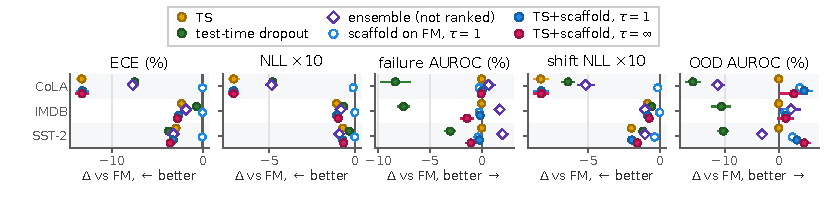
\includegraphics[width=\linewidth]{fig_fn_nlp_delta.pdf}
  \par\smallskip\raggedright\small
  \begin{itemize}
    \item ECE, TS vs TS+scaffold: CoLA $4.69$ vs $4.77$, IMDB $1.69$ vs $1.39$, SST-2 $2.84$ vs $2.53$. NLL equal.
    \item OOD (entropy AUROC): CoLA $73.4\to78.1$, SST-2 $84.5\to87.8$, IMDB $92.2\to93.5$ (within error).
  \end{itemize}
  \source{Change vs the FM, mean $\pm$ s.e.\ over 5 seeds.}
\end{frame}

% ============================================================ 5
\begin{frame}{SST-2 vs DIRECTOR Table 7}
  \centering
  \small
  \begin{tabular}{@{}lcccc@{}}
    \toprule
    SST-2, Qwen2.5-0.5B & ACC & ECE$\downarrow$ & NLL$\times10\downarrow$ & Brier$\downarrow$\\
    \midrule
    Qwen2.5 (DIRECTOR T7) & 93.01 & 5.86 & 3.30 & 12.18\\
    DIRECTOR, last 3 blocks (T7) & 93.12 & 5.48 & 2.95 & 12.09\\
    \midrule
    Our FM (5 seeds) & 92.62 & 5.77 & 2.71 & 12.88\\
    \quad + TS & 92.62 & 2.84 & 1.98 & \textbf{11.31}\\
    \quad + TS + scaffold & 92.63 & \textbf{2.53} & \textbf{1.97} & 11.39\\
    \bottomrule
  \end{tabular}
  \par\medskip\raggedright
  \begin{itemize}
    \item Same starting point (ECE $5.77$ vs $5.86$).
    \item TS alone: ECE $-2.9$. DIRECTOR: $-0.38$.
    \item T7 has no TS row: TS on top of DIRECTOR is still open.
  \end{itemize}
\end{frame}

% ============================================================ 6
\begin{frame}{Held-out calibration}
  \centering
  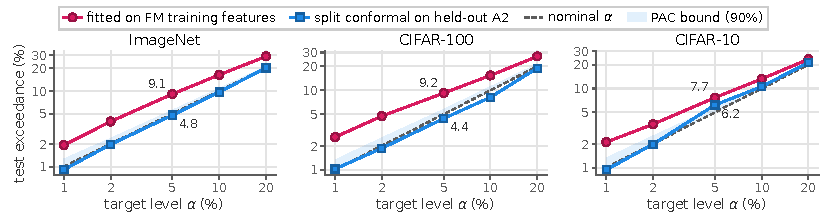
\includegraphics[width=0.92\linewidth]{fig_fn_train_vs_heldout.pdf}
  \par\smallskip\raggedright\small
  \begin{itemize}
    \item Threshold at $\alpha=5\%$ fitted on training features: $9.1\%$ exceedance on ImageNet, $9.2\%$ on CIFAR-100. On held-out data: $4.8\%$, $4.4\%$.
    \item Splits: A1 (learn) / A2 (conformal) / calB (certify) / calC (label sets) / test. ImageNet: 2.5k / 2.5k / 5k / 10k / 30k of the 50k val images.
  \end{itemize}
\end{frame}

% ============================================================
\section{Full ImageNet}

% ============================================================ 7
\begin{frame}{Full ImageNet: setup}
  \small
  \begin{itemize}
    \item \textbf{FM:} ViT-B/16 (in21k $\to$ in1k), top-1 $81.7\%$.
    \item \textbf{Compile} (Thrust 1, Eq.~7): flow matching on \textbf{all 1.28M} training images, 60k steps.
      \begin{itemize}\small
        \item Last 4 blocks, and all 12 blocks.
        \item Control arms: 100k and 318k images; 1.28M with a 15k-step schedule.
      \end{itemize}
    \item \textbf{Fidelity:} top-1 / top-5 agreement with the FM, KL, accuracy (10k val images).
    \item \textbf{Uncertainty:} DIRECTOR's metrics on val, ImageNet-C (4 corruptions), OOD (ImageNet-O, Textures, noise).
  \end{itemize}
\end{frame}

% ============================================================ 8
\begin{frame}{Last 4 blocks: 80.7\% agreement}
  \centering
  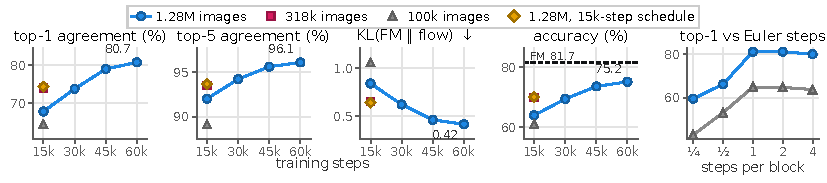
\includegraphics[width=\linewidth]{fig_fn_full_compile.pdf}
  \par\smallskip\raggedright\small
  \begin{itemize}
    \item Top-1 agreement $80.7\%$, top-5 $96.1\%$, KL $0.42$, accuracy $75.2$ (FM $81.7$). Before: $74.0\%$ (318k images).
    \item \textbf{Steps, not data:} 1.28M images at 15k steps $=74.3\%$, same as 318k.
    \item Stable from 1 Euler step per block: $81.0 / 81.0 / 79.9\%$ at 1 / 2 / 4 steps.
  \end{itemize}
\end{frame}

% ============================================================ 9
\begin{frame}{All 12 blocks: 45\% agreement}
  \centering
  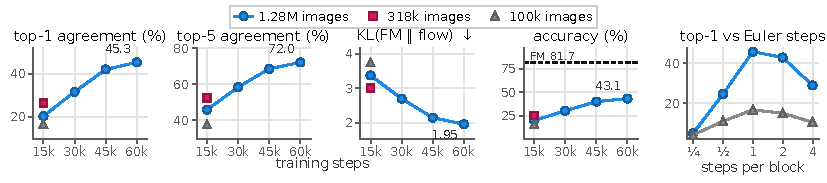
\includegraphics[width=\linewidth]{fig_fn_full_compile_all12.pdf}
  \par\smallskip\raggedright\small
  \begin{itemize}
    \item Top-1 agreement $45.3\%$, top-5 $72.0\%$, KL $1.95$, accuracy $43.1$ (FM $81.7$).
    \item Still rising but slowly: $20.2 \to 31.5 \to 42.0 \to 45.3\%$ at 15k / 30k / 45k / 60k steps.
    \item Not a convergent ODE: $45.9 \to 42.9 \to 28.9\%$ at 1 / 2 / 4 steps per block.
  \end{itemize}
\end{frame}

% ============================================================ 10
\begin{frame}{Uncertainty on the compiled flow}
  \centering
  \small
  \begin{tabular}{@{}llccccc@{}}
    \toprule
    & & ACC & NLL$\downarrow$ & ECE$\downarrow$ & Shift NLL$\downarrow$ & OOD AUROC\\
    \midrule
    & FM (reference) & \textbf{81.68} & \textbf{0.694} & 4.00 & \textbf{1.401} & \textbf{0.915}\\
    \midrule
    \multirow{4}{*}{Last 4} & Flow & 75.19 & 0.950 & 2.17 & 1.743 & 0.842\\
    & + TS & 75.19 & 0.950 & \textbf{1.66} & 1.747 & 0.846\\
    & + scaffold, $\tau=1$ & 75.12 & 0.959 & 1.84 & 2.010 & 0.877\\
    & + scaffold, $\tau=\infty$ & 75.15 & 0.991 & 2.81 & 2.554 & 0.909\\
    \midrule
    \multirow{3}{*}{All 12} & Flow & 43.17 & 2.503 & 3.04 & 4.792 & 0.546\\
    & + TS & 43.17 & 2.496 & 1.07 & 4.876 & 0.524\\
    & + scaffold (not certified) & 43.05 & 2.539 & 3.85 & 4.904 & 0.825\\
    \bottomrule
  \end{tabular}
  \par\medskip\raggedright
  \begin{itemize}
    \item Last 4: scaffold brings OOD close to the FM ($0.842\to0.909$), but shift NLL rises.
    \item All 12: the flow is more confident on noise than on images; LTT certifies none of the 40 candidates (flips $\ge0.78\%$).
  \end{itemize}
\end{frame}

% ============================================================ 11
\begin{frame}{ImageNet FM in DIRECTOR's metrics}
  \centering
  \small
  \begin{tabular}{@{}lcccccc@{}}
    \toprule
    & \multicolumn{3}{c}{In distribution} & \multicolumn{2}{c}{Shift} & OOD\\
    \cmidrule(lr){2-4}\cmidrule(lr){5-6}\cmidrule(lr){7-7}
    ViT-B/16 & ACC & ECE$\downarrow$ & NLL$\times10\downarrow$ & ACC & NLL$\times10\downarrow$ & AUROC\\
    \midrule
    FM & 81.68 & 4.00 & 6.94 & 67.05 & 14.01 & 91.5\\
    TS & 81.68 & 2.95 & 6.92 & 67.05 & 13.97 & 92.0\\
    MC dropout & \textbf{82.11} & \textbf{1.90} & \textbf{6.58} & 66.94 & \textbf{13.80} & 91.5\\
    \midrule
    TS + scaffold, $\tau=1$ & 81.69 & 2.63 & 6.98 & 66.11 & 16.07 & 93.9\\
    TS + scaffold, $\tau=\infty$ & 81.33 & 4.46 & 7.68 & 51.04 & 33.30 & \textbf{95.1}\\
    \midrule
    {\color{inkgrey}Ensemble (3$\times$ cost)} & {\color{inkgrey}85.50} & {\color{inkgrey}5.12} & {\color{inkgrey}5.63} & {\color{inkgrey}76.05} & {\color{inkgrey}10.31} & {\color{inkgrey}92.3}\\
    \bottomrule
  \end{tabular}
  \par\medskip\raggedright
  \begin{itemize}
    \item In distribution: ties TS. OOD: $+2$ to $+3.5$ AUROC.
    \item Shift is not covered by the ID certificate: $\tau=\infty$ drops shift accuracy $67\to51$.
  \end{itemize}
  \source{OOD: entropy AUROC, mean over ImageNet-O, Textures, noise. One checkpoint, no error bars.}
\end{frame}

% ============================================================
\section{Input-specific uncertainty}

% ============================================================ 12
\begin{frame}{Input $\to$ conformal $\to$ threshold $\to$ rate}
  \centering
  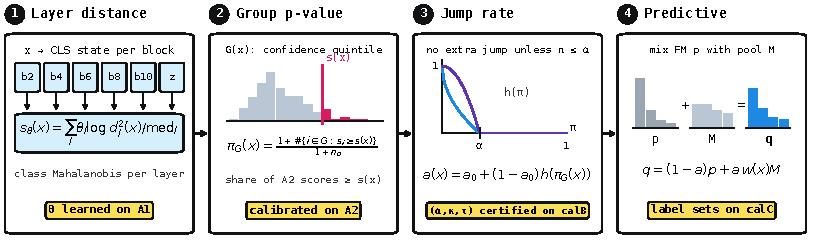
\includegraphics[width=\linewidth]{fig_fn_pipeline_method.pdf}
  \par\medskip\raggedright\small
  \[
    a(\x)=a_0+(1-a_0)\,h\big(\pi_{G}(\x)\big),\qquad
    q(\cdot\mid\x)=(1-a(\x))\,p(\cdot\mid\x)+a(\x)\,w(\x)M .
  \]
  An input pays nothing unless its group p-value is below $\alpha$. One score for all layers: $\alpha$ instead of $L\alpha$.
\end{frame}

% ============================================================ 13
\begin{frame}{What is learned, and where}
  \small
  \begin{tabular}{@{}p{0.2\linewidth}p{0.1\linewidth}p{0.62\linewidth}@{}}
    \toprule
    Quantity & Split & How\\
    \midrule
    Distance $\theta$ & A1 & logistic regression of FM errors on layer distances ($\theta\ge0$), or uniform\\
    Threshold $\hat b_G$ & A2 & conformal quantile per group: not tuned, fixed by $\alpha$\\
    $(\alpha,\kappa,\tau)$ & calB & Learn-then-Test over 40 candidates: flip $\le1\%$, jump $\le5\%$, $\delta=0.1$; take the most sensitive\\
    \bottomrule
  \end{tabular}
  \par\bigskip
  \begin{block}{Why not learn $b$ by likelihood}
    If the FM is calibrated, every scaffold has $\E[-\log q]\ge\E[-\log p]$ (Gibbs), so the NLL-optimal $b$ is $+\infty$.\\
    Observed: no jump at all on ImageNet and CIFAR-100; jumps on $99.8\%$ of CoLA (a worse TS).
  \end{block}
\end{frame}

% ============================================================ 14
\begin{frame}{Input-level guarantees}
  \small
  \textbf{Not possible:} exact per-input coverage forces trivial sets (Vovk 2012; Barber et al.\ 2021).\\
  \textbf{Possible:} per group $G$ of inputs (FM confidence quintile), computed from $\x$ alone.
  \par\medskip
  \begin{tabular}{@{}lll@{}}
    \toprule
    & Guarantee (per group $k$) & Split\\
    \midrule
    A & $P(s(X)>\hat b_k\mid G=k)\le\alpha$ & A2\\
    B & $\E[\mathrm{TV}(q,p)\mid G=k]\le a_0+(1-a_0)\,\alpha\kappa/(\kappa+1)$ & A2\\
    C & $P(\text{flip}\mid G=k)\le\alpha+P(\text{margin}\le a_0/(1-a_0))$ & A2\\
    D & $P(Y\in C(X)\mid G=k)\ge1-\alpha$ (label sets) & calC\\
    E & PAC version of A, Beta quantile over A2 & A2\\
    F & flip $\le1\%$ and jump $\le5\%$ w.p.\ $\ge0.9$ (LTT) & calB\\
    \bottomrule
  \end{tabular}
  \source{Price of small groups: slack $1/(n_G+1)$. CoLA has $n_G\approx45$, so $\alpha=1\%$ is out of reach.}
\end{frame}

% ============================================================ 15
\begin{frame}{Marginal vs per group}
  \centering
  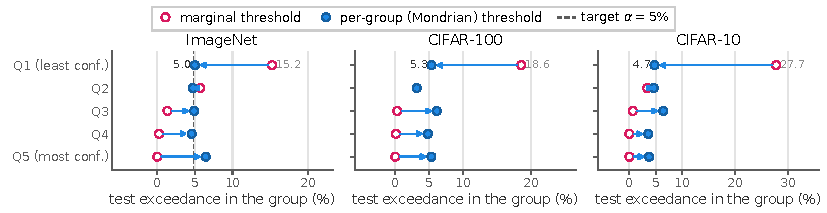
\includegraphics[width=\linewidth]{fig_fn_group_exceedance.pdf}
  \par\smallskip\raggedright\small
  \begin{itemize}
    \item Marginal $\alpha=5\%$ is violated on the least confident inputs: $15.2\%$ (ImageNet), $18.6\%$ (C100), $27.7\%$ (C10).
    \item Per group: $4.6$--$6.5\%$ on ImageNet.
  \end{itemize}
\end{frame}

% ============================================================ 16
\begin{frame}{Certified strength}
  \centering
  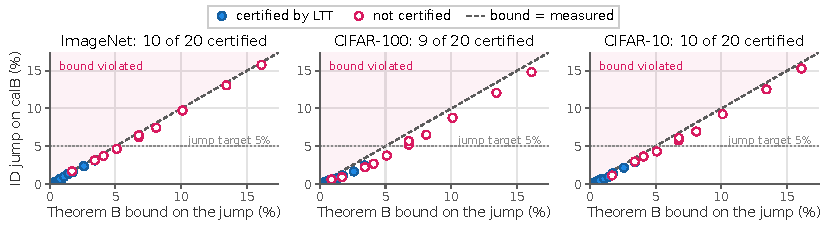
\includegraphics[width=\linewidth]{fig_fn_ltt_budget.pdf}
  \par\smallskip\raggedright\small
  \begin{itemize}
    \item Measured jump mass never exceeds the bound of B, on every candidate.
    \item LTT certifies 21--23 of 40 per dataset. Small calB (CoLA, 454): Bonferroni certifies none, fixed-sequence testing 22.
  \end{itemize}
\end{frame}

% ============================================================
\section{Novelty and position}

% ============================================================ 17
\begin{frame}{What is new vs Thrust 1}
  \footnotesize
  \renewcommand{\arraystretch}{1.15}
  \begin{tabular}{@{}>{\raggedright\arraybackslash}p{0.25\linewidth}>{\raggedright\arraybackslash}p{0.39\linewidth}>{\raggedright\arraybackslash}p{0.30\linewidth}@{}}
    \toprule
    Thrust 1 as written & Ours & Evidence\\
    \midrule
    Compile blocks (Eq.~7) & Kept; fidelity reported first & IN last 4: $80.7\%$, all 12: $45\%$\\
    Brownian SDE + score drift (Eq.~5) & Regeneration: exact layer marginals, any rate, no score model & Brownian: no gain over TS\\
    Variance prior (Eq.~8) & Rate from a conformal p-value of a multi-layer distance & Eq.~8: AUROC $0.14$; distance: $0.97$ (pilot)\\
    Quadrature recursion (Eq.~6) & Closed-form predictive & One forward pass\\
    Wasserstein refinement (Eq.~9) & LTT certificate on held-out data & 21--23 / 40 certified\\
    No input-level guarantee & Group-conditional guarantees A--F & Worst group $15$--$28\%\to5\%$\\
    \bottomrule
  \end{tabular}
  \source{Eq.~6's $\epsilon$ assumes a convergent ODE; the compiled field behaves as a per-block map.}
\end{frame}

% ============================================================ 18
\begin{frame}{Where it stands}
  \small
  \begin{itemize}
    \item \textbf{Works:} guarantees hold where splits are exchangeable; accuracy kept; OOD better than the softmax.
    \item \textbf{Ceiling:}
      \begin{itemize}\small
        \item ID calibration $\le$ TS: mixing towards $M$ is the only action.
        \item The distance measures atypicality, not error: error AUROC $0.761$ vs softmax $0.874$ (ImageNet).
        \item OOD of $q$ stays below the distance itself (ImageNet far OOD $97.0$).
        \item Shift: OOD gains cost shift NLL.
      \end{itemize}
  \end{itemize}
  \medskip
  \centering
  \fbox{\parbox{0.8\linewidth}{\centering ID calibration $\approx$ TS,\quad OOD $\approx$ max(softmax, distance)}}
\end{frame}

% ============================================================ 19
\begin{frame}{Option 1: TS + conformal flag}
  \centering
  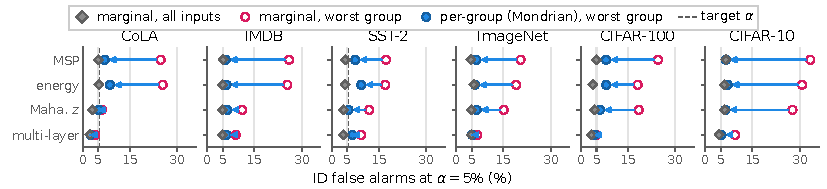
\includegraphics[width=\linewidth]{fig_fn_flag_validity.pdf}
  \par\smallskip\raggedright\small
  \begin{itemize}
    \item TS for probabilities, a separate flag for atypical inputs. False alarms $\le\alpha$, also per group.
    \item ImageNet, $\alpha=5\%$, multi-layer distance: false alarms $4.6\%$ (worst group $5.1\%$; MSP flag $20.5\%$). Flags ImageNet-O $43\%$, Textures $80\%$, noise $100\%$.
  \end{itemize}
  \source{Modest novelty: conformal outlier tests exist. New: per-group guarantee, combination with TS, DIRECTOR's benchmarks.}
\end{frame}

% ============================================================ 20
\begin{frame}{Questions for you}
  \small
  \begin{enumerate}
    \item \textbf{Direction:} continue the scaffold (ties TS, OOD gains) or move to Option 1 (TS + flag)?
    \item \textbf{Marginal preservation:} replace exact preservation by the certified bound
      \[ \|\E_X q(\cdot\mid X)-\E_X p(\cdot\mid X)\|_{\mathrm{TV}}\le a_0+(1-a_0)\tfrac{\alpha\kappa}{\kappa+1}\ \text{(ID)}? \]
    \item \textbf{Compile:} is $80.7\%$ (last 4) enough? Longer run, or 318k images at 60k steps to separate data from steps?
  \end{enumerate}
  \medskip
  \textbf{Running:} DIRECTOR reproduction with the authors' code, 335 / 450 runs.
\end{frame}

% ============================================================
\appendix

\begin{frame}{Backup: vision, change vs FM}
  \centering
  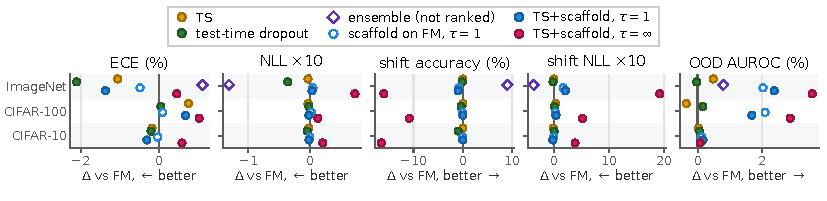
\includegraphics[width=\linewidth]{fig_fn_vision_delta.pdf}
  \par\smallskip\raggedright\small
  ImageNet, CIFAR-100, CIFAR-10; one checkpoint each.
\end{frame}

\begin{frame}{Backup: label sets}
  \centering
  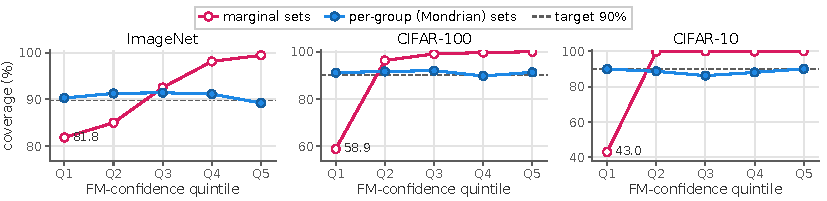
\includegraphics[width=\linewidth]{fig_fn_label_sets.pdf}
  \par\smallskip\raggedright\small
  Target $90\%$. Least confident quintile: marginal $81.8 / 58.9 / 43.0\%$, per group $90.3 / 91.1 / 89.9\%$ (IN / C100 / C10). The gain comes from Mondrian, not the scaffold.
\end{frame}

\end{document}
